\documentclass[aspectratio=1610]{beamer}
\usepackage[T1]{fontenc}
\usetheme{wildcat}
\usetikzlibrary{arrows.meta,angles,quotes,calc,intersections,positioning}

\usepackage{amsmath,amssymb,amsfonts}
\usepackage{booktabs}
\usepackage{relsize}
\usepackage{pgfplots}
\pgfplotsset{compat=1.16}
\usepackage{array}
\usepackage{siunitx}
\usepackage{cancel}
\usepackage{jupyter}
\usepackage{minted}

\let\oldfootnotesize\footnotesize
\renewcommand*{\footnotesize}{\oldfootnotesize\tiny}

\def\mathdefault#1{#1}
\everymath=\expandafter{\the\everymath\displaystyle}


\title{Designing a PWR Unit Cell  \\
       {\small\it NE 630 - Lecture 19}}

\date{\input{term.txt} \\ {\footnotesize Git SHA: \input{git_sha.txt}}}

\author{Jeremy Roberts}


\definecolor{ksupurple}{HTML}{512888}
\definecolor{orange}{HTML}{CA7C1B}
\definecolor{skyblue}{RGB}{180,220,255}

\begin{document}

\begin{frame}
\titlepage
\end{frame}
 
 
%%%%%%%%%%%%%%%%%%%%%%%%%%%%%%%%%%%%%%%%%%%%%%%%%%%
\begin{frame}{Primary Objective}

Students will be able to 

\vfill

\begin{quote}
\textcolor{wcprimary}{construct a detailed model of a LWR unit cell
and compare the results to theoretical models based on the four-factor formula.
}
\end{quote}

\vfill 

\end{frame}

%%%%%%%%%%%%%%%%%%%%%%%%%%%%%%%%%%%%%%%%%%%%%%%%%%%%%%%%%%%%%%%%%%%%%%%%%%%%%%
\begin{frame}{Review: the four-factor formula}

Recall $k_{\infty} = \eta_T f p \varepsilon$, where
\begin{align*}
\eta_T &= \frac{\nu\bar{\Sigma}_{fT}^f} {\bar{\Sigma}^f_{aT}} \\
f &= \frac{1}{1 + \zeta \left(V_{nf} \bar{\Sigma}^{nf}_{aT} \big/ V_f \bar{\Sigma}^f_{aT} \right ) } \\
p &= 1 - \frac{V_f \bar{\Sigma}^f_{aF} \bar{\phi}^{f}_{F}}
      {V_f \left[ \bar{\Sigma}^f_{aT} \bar{\phi}^{f}_{T} + \bar{\Sigma}^f_{aF} \bar{\phi}^{f}_{F} \right ]+ V_{nf} \bar{\Sigma}^{nf}_{aT} \bar{\phi}^{nf}_{T}} 
  \approx \textcolor{wcprimary}{\exp \left (- \frac{V_f  N_{fe} I^{\text{het}}_a}{V_{m} \xi^{m} \Sigma^{m}_s  } \right )} \\
\varepsilon &= \frac{\nu\bar{\Sigma}^f_{fT} \bar{\phi}^{f}_{T} + \nu\bar{\Sigma}^f_{fF} \bar{\phi}^{f}_{F} }
   {\nu\bar{\Sigma}^f_{fT} \bar{\phi}^{f}_{T} } 
 \approx \textcolor{wcprimary}{ 1 + \frac{ (1-\tilde{e})}{\tilde{e}} \frac{\bar{\nu}^{fe} \bar{\sigma}^{fe}_{fF} }
                     {\bar{\nu}^{fi}\bar{\sigma}^{fi}_{fT}   }}
\end{align*}

\vfill 

Here, ${}^f$ and ${}^{nf}$ indicate ``fuel'' and ``non-fuel'', $_T$ and $_F$ indicate ``thermal'' and ``non-thermal'' (or $E > 1$ eV), and $\bar{\,}$ indicates averaging over space and/or energy.
\end{frame}



%%%%%%%%%%%%%%%%%%%%%%%%%%%%%%%%%%%%%%%%%%%%%%%%%%%%%%%%%%%%%%%%%%%%%%%%%%%%%%
\begin{frame}{Designing a PWR Unit Cell in OpenMC}

\begin{columns}[T,onlytextwidth]
% ----------------------------------------------------------
\begin{column}{0.45\textwidth}
\centering
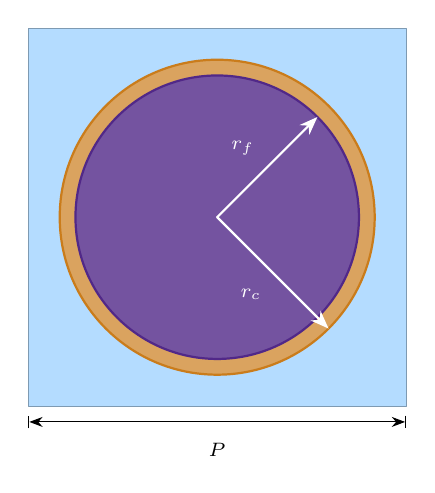
\begin{tikzpicture}[>=Stealth, line cap=round, line join=round, scale=4]

% --- Parameters (cm) ---
\def\P{1.2}       % pitch
\def\rfuel{0.45}  % fuel radius
\def\rclad{0.50}  % cladding outer radius
\def\halfP{0.6}   % P/2

% --- Colors (for standalone compilation) ---
\definecolor{skyblue}{RGB}{180,220,255}
\definecolor{wcprimary}{HTML}{512888}
\definecolor{wcalerted}{HTML}{CA7C1B}

% --- Background water ---
\fill[skyblue, draw=skyblue!70!black, thin] (-\halfP,-\halfP) rectangle (\halfP,\halfP);

% --- Cladding and fuel ---
\filldraw[wcalerted, fill=wcalerted!70, thick] (0,0) circle (\rclad);
\filldraw[wcprimary, fill=wcprimary!80, thick] (0,0) circle (\rfuel);

% --- Dimension arrows ---
\def\angfuel{45}
\def\angclad{-45}

% Fuel radius arrow
\draw[->, thick, white]
  (0,0) -- ++(\angfuel:\rfuel)
  node[midway, above left=0.5pt and 1pt, font=\scriptsize, text=white]
  {$r_f$};

% Cladding radius arrow
\draw[->, thick, white]
  (0,0) -- ++(\angclad:\rclad)
  node[midway, below left=2pt and 0.5pt, font=\scriptsize, text=white]
  {$r_c$};

% Pitch label (bottom)
\draw[|<->|]
  (-\halfP,-\halfP-0.05) -- (\halfP,-\halfP-0.05)
  node[midway, below=4pt, font=\scriptsize] {$P$};

\end{tikzpicture}
\end{column}

% ----------------------------------------------------------
\begin{column}{0.55\textwidth}
\small

\begin{table}
\begin{tabular}{ccc}
\toprule
 {\bf Region} & {\bf ``Volume''} & {\bf Material} \\
\midrule
 \textcolor{wcprimary}{Fuel} &  \textcolor{wcprimary}{$\pi r_f^2$} &  \textcolor{wcprimary}{(enriched) UO$_2$} \\
\midrule
 \textcolor{wcalerted}{Cladding}  & \textcolor{wcalerted}{$\pi (r_c^2 - r_f^2)$} & \textcolor{wcalerted}{Zircaloy-4}\\
\midrule
 Moderator  & $P^2 - \pi r_c^2$ & (borated) water\\
\bottomrule
\end{tabular}
\end{table}

\vspace{0.25cm}

{\bf The Initial Goal}: Given $r_f$ and $r_c$, determine $P$ such that
we maximize $k_{\infty}$.  Equivalently, find the value of $P/D$ that maximizes $k_{\infty}$, where $D$ is the fuel diameter.

\vspace{0.25cm}

{\bf Ponderables}: Which of the four factors depend on $r_f$ and $P$, or, equivalently, $P/D$?
What range of values can $P/D$ have?

\end{column}
% ----------------------------------------------------------
\end{columns}

\end{frame}

%%%%%%%%%%%%%%%%%%%%%%%%%%%%%%%%%%%%%%%%%%%%%%%%%%%%%%%%%%%%%%%%%%%%%%%%%%%%%%
\begin{frame}[fragile]{Model Initialization and Parameters}

\begin{minted}[frame=single,framesep=5pt]{python}
import numpy as np, matplotlib.pyplot as plt, openmc
model = openmc.Model()
enrichment = 4.0   # % by atom
fuel_radius = 0.45 # cm
clad_radius = 0.46 # cm
pitch = 1.2        # cm
enrichment = 4.0   # weight percent
boron_ppm = 0.0    # parts per million 
pressure = 15.5    # MPa
T_fuel = 1200.0    # K
T_cool = 600.0     # K
# volumes for each region 
fuel_volume = np.pi*fuel_radius**2 
clad_volume = np.pi*clad_radius**2 - fuel_volume
cool_volume = pitch**2 - np.pi*clad_radius**2
\end{minted}

\end{frame}
  
%%%%%%%%%%%%%%%%%%%%%%%%%%%%%%%%%%%%%%%%%%%%%%%%%%%%%%%%%%%%%%%%%%%%%%%%%%%%%%
\begin{frame}[fragile]{Model Materials}

\begin{minted}[frame=single,framesep=5pt]{python}
uo2 = openmc.Material(name="uo2")
uo2.add_element('U', 1.0, enrichment=enrichment)
uo2.add_element('O', 2.0)
uo2.set_density('g/cc', 10.5)
uo2.temperature = T_fuel
# Zircaloy-4 has < 2% Fe, Cr, and Sn
zirconium = openmc.Material(name="zirconium")
zirconium.add_element('Zr', 1.0)
zirconium.set_density('g/cc', 6.6)
zirconium.temperature = 0.5*(T_fuel + T_cool)
# Helper function automatically computes density
water = openmc.model.borated_water(
  boron_ppm=boron_ppm, temperature=T_cool, temp_unit='K',
  pressure=pressure,  press_unit='MPa')
model.materials = [uo2, zirconium, water]
\end{minted}

\end{frame}

%%%%%%%%%%%%%%%%%%%%%%%%%%%%%%%%%%%%%%%%%%%%%%%%%%%%%%%%%%%%%%%%%%%%%%%%%%%%%%
\begin{frame}[fragile]{Model Geometry}

\begin{minted}[frame=single,framesep=5pt]{python}
fuel_surface = openmc.ZCylinder(r=fuel_radius)
clad_surface = openmc.ZCylinder(r=clad_radius)
outer_surface = openmc.model.RectangularPrism(
  width=pitch, height=pitch, boundary_type='reflective')  
fuel_region = -fuel_surface
clad_region = +fuel_surface & -clad_surface
cool_region = +clad_surface & -outer_surface          
fuel_cell = openmc.Cell(name='fuel', 
  fill=uo2, region=fuel_region)
clad_cell = openmc.Cell(name='cladding', 
  fill=zirconium, region=clad_region)
cool_cell = openmc.Cell(name='coolant', 
  fill=water, region=cool_region)
root_universe = openmc.Universe(
  cells=(fuel_cell, clad_cell, cool_cell))
model.geometry.root_universe = root_universe
\end{minted}

\end{frame}

%%%%%%%%%%%%%%%%%%%%%%%%%%%%%%%%%%%%%%%%%%%%%%%%%%%%%%%%%%%%%%%%%%%%%%%%%%%%%%
\begin{frame}[fragile]{Model Source and Settings}

\begin{minted}[frame=single,framesep=5pt]{python}
# distributions in space, angle, and energy
d_space = openmc.stats.Point((0, 0, 0))
d_angle = openmc.stats.Isotropic()
d_energy = openmc.stats.Watt()
# initial neutron distribution
source = openmc.IndependentSource(
  space=d_space, angle=d_angle, energy=d_energy)
# settings that govern simulation
model.settings.batches = 100    # number of "generations"
model.settings.inactive = 10    # number to skip
model.settings.particles = 1000 # number of n's per "gen"
model.settings.run_mode = 'eigenvalue' # solve for k_oo
model.settings.temperature = {"method": "interpolation"}
\end{minted}

\end{frame}

%%%%%%%%%%%%%%%%%%%%%%%%%%%%%%%%%%%%%%%%%%%%%%%%%%%%%%%%%%%%%%%%%%%%%%%%%%%%%%
\begin{frame}[fragile]{Model Tallies (i.e., What We Compute Beyond $k_{\infty}$)}

The following sets up the computation of $\phi_{g}^{R}$ for 
\begin{itemize}
 \item $R \in \{\text{fuel, cladding, moderator} \}$
 \item $g \in \{ 1, 2, \ldots, G=70 \}$
\end{itemize}
Explore {\tt openmc.mgxs.GROUP\_STRUCTURES} for other options.
 
\begin{minted}[frame=single,framesep=5pt]{python}
spectrum_bounds = openmc.mgxs.GROUP_STRUCTURES["CASMO-70"]
energy_filter = openmc.EnergyFilter(spectrum_bounds)
cell_filter = openmc.CellFilter(
  [fuel_cell, clad_cell, cool_cell])
spectrum_tally = openmc.Tally()
spectrum_tally.filters = [cell_filter, energy_filter]
spectrum_tally.scores = ['flux']
model.tallies.append(spectrum_tally)
\end{minted}

\end{frame}

%%%%%%%%%%%%%%%%%%%%%%%%%%%%%%%%%%%%%%%%%%%%%%%%%%%%%%%%%%%%%%%%%%%%%%%%%%%%%%
\begin{frame}[fragile]{Multigroup Cross Sections}

The following sets up the computation of $\bar{\Sigma}_{x,g}^{R}$, etc., for 
\begin{itemize}
 \item $R \in \{\text{fuel, cladding, moderator} \}$
 \item $g \in \{ 1, 2, \ldots, G=70 \}$
 \item $x \in \{t, a, f, s \}$, etc.
\end{itemize}
 
\begin{minted}[frame=single,framesep=5pt]{python}
mgxs_lib = openmc.mgxs.Library(model.geometry)
mgxs_lib.energy_groups = \
  openmc.mgxs.EnergyGroups(group_edges=[1e-3,1,1e7])
mgxs_lib.mgxs_types = ['total', 'absorption', 'nu-fission', 
  'fission', 'scatter matrix', 'chi']
mgxs_lib.domain_type = 'cell'
mgxs_lib.domains = \
  model.geometry.get_all_material_cells().values()
mgxs_lib.by_nuclide = False # True for microscopic 
mgxs_lib.build_library()
mgxs_lib.add_to_tallies_file(model.tallies, merge=True)
\end{minted}

\end{frame}

%%%%%%%%%%%%%%%%%%%%%%%%%%%%%%%%%%%%%%%%%%%%%%%%%%%%%%%%%%%%%%%%%%%%%%%%%%%%%%
\begin{frame}[fragile]{Running Simulation and Loading Results}


\begin{minted}[frame=single,framesep=5pt]{python}
# Run the model and return the statepoint (result file) path
sp_path = model.run(output=True)

# Load the results and cross sections
sp = openmc.StatePoint(sp_path)
mgxs_lib.load_from_statepoint(sp)

# OpenMC places all the values in a 1-D array.  Reshaping 
# and transposing gives us a 2-D array with the multigroup 
# flux for each of the 3 regions by column.
phi = sp.tallies[spectrum_tally.id].mean.reshape((3, 
  len(spectrum_bounds)-1)).T
\end{minted}

\end{frame}

%%%%%%%%%%%%%%%%%%%%%%%%%%%%%%%%%%%%%%%%%%%%%%%%%%%%%%%%%%%%%%%%%%%%%%%%%%%%%%
\begin{frame}[fragile]{Processing the Spectra}

The fluxes computed by OpenMC are actually equal to $V^R \phi^R_g$.  In short,
OpenMC tracks neutrons and, by group and region, adds up the total distance 
all neutrons travel.  This gives a unit of [cm] (per source particle).  To get 
the per cm$^2$, we need to divide by volume.  To get per $eV$, we further divide 
by the group widths.  The per s depends on our assumed source strength, which 
would have to be scaled to some known fission rate or power.

\begin{minted}[frame=single,framesep=5pt]{python}
# Define the group widths 
dE = np.diff(spectrum_bounds)

# Divide by the region volume and group widths
phi_fuel = phi[:, 0]/dE/fuel_volume
phi_clad = phi[:, 1]/dE/clad_volume
phi_cool = phi[:, 2]/dE/cool_volume
\end{minted}

\end{frame}

%%%%%%%%%%%%%%%%%%%%%%%%%%%%%%%%%%%%%%%%%%%%%%%%%%%%%%%%%%%%%%%%%%%%%%%%%%%%%%
\begin{frame}[fragile]{Processing the Multigroup Cross Sections}

Now, collect the two-group data into a form for easily computing the four factors:

\begin{minted}[frame=single,framesep=5pt]{python}
# Place volumes and cells in dictionary
V = {"fuel": fuel_volume, "clad": clad_volume, 
  "cool": cool_volume}
cells = {"fuel": fuel_cell, "clad": clad_cell, 
  "cool": cool_cell}

# Extract region-wise, multigroup parameters
φ = {}; Σ_a = {}; νΣ_f = {}
for R in ["fuel", "clad", "cool"]:
  φ[R] = mgxs_lib.get_mgxs(cells[R],"total").get_flux()/V[R]
  Σ_a[R] = mgxs_lib.get_mgxs(cells[R],"absorption").get_xs()
  νΣ_f[R] = mgxs_lib.get_mgxs(cells[R],"nu-fission").get_xs()
# Now, e.g., the thermal fuel flux is φ["fuel"][1] while 
# the fast (or non-thermal) absorption cross section is 
# Σ_a["fuel"][0]
\end{minted}


\end{frame}
 
%%%%%%%%%%%%%%%%%%%%%%%%%%%%%%%%%%%%%%%%%%%%%%%%%%%%%%%%%%%%%%%%%%%%%%%%%%%%%%
\begin{frame}[fragile]{Computing the Four Factors and $k_{\infty}$}

To keep things tidy, start by defining volume-integrated reaction rates.  
For example, the total rate of thermal absorption in the moderator is
\begin{minted}[frame=single,framesep=5pt]{python}
R_a_m_T = V["cool"]*φ["cool"][1]*Σ_a["cool"][1]
# do also for R_a_m_F, R_a_c_T, ..., R_n_f_T, R_a_f_F
\end{minted}
where, e.g., {\tt R\_n\_f\_T} indicates the neutron generation rate in the fuel 
from fission due to thermal neutrons.  
Then, define  {\tt R\_a\_nf\_T} and   {\tt R\_a\_nf\_T} for non-fuel 
absorption rates.  
Finally, define the four factors
\begin{minted}[frame=single,framesep=5pt]{python}
η_T =
f = 
p = 
ε =
\end{minted}
from which 
\begin{minted}[frame=single,framesep=5pt]{python}
k_oo =
\end{minted}

\end{frame}

%%%%%%%%%%%%%%%%%%%%%%%%%%%%%%%%%%%%%%%%%%%%%%%%%%%%%%%%%%%%%%%%%%%%%%%%%%%%%%
\begin{frame}[fragile]{Back to $P/D$ and Maximizing $k_{\infty}$}

Although OpenMC models can be set up with loops over geometric or material 
properties, the Jupyter notebook is not the ideal environment.  A simpler 
approach that is less prone to user errors is simply to 
\begin{enumerate}
 \item Set the desired value for, e.g., $P = P_0$.
 \item Restart the Kernel and Run All 
 \item Record the desired outputs.
 \item Repeat for $P = P_1, P_2, \ldots$.
\end{enumerate}

 

\end{frame}

%%%%%%%%%%%%%%%%%%%%%%%%%%%%%%%%%%%%%%%%%%%%%%%%%%%%%%%%%%%%%%%%%%%%%%%%%%%%%%
\begin{frame}[fragile]{Looping OpenMC Runs}

For automating with loops, I recommend writing a Python file of the form 
\begin{minted}[frame=single,framesep=5pt]{python}
# my_model.py
import openmc
def run_it(P):
  model = openmc.Model()
  ...
  pitch = P
  ...
  return η_T, f, p, ε
\end{minted}

Then, in Jupyter, you can do things like 

\begin{minted}[frame=single,framesep=5pt]{python}
import my_model 
for P in [1.1, 1.3, 1.5]:
  η_T, f, p, ε = my_model.run_it(P)
  # do whatever you want to do with these!
\end{minted}

\end{frame}

%%%%%%%%%%%%%%%%%%%%%%%%%%%%%%%%%%%%%%%%%%%%%%%%%%%%%%%%%%%%%%%%%%%%%%%%%%%%%%
\begin{frame}[fragile]{Some Exploratory Exercises}

Given this basic model, you can now provide quantitative answers to 
questions like... 
\begin{enumerate}
 \item What $P$ maximizes $k_{\infty}$?
 \item How do the four factors vary with $P/D$?
 \item How do the answers to (1) and (2) change if we put 800 ppm of boron in the coolant?
 \item What happens to the four factors and $k_{\infty}$ if we replace our (light) water 
       with heavy water?  Graphite?  Does $k_{\infty}$ peak at the same $P/D$?
 \item What happens to $k_{\infty}$ if we replace the zirconium with stainless steel?  
       SiC?
 \item If our 3400 MW$_{\text{th}}$ reactor has 50,000 of these rods (3 m in length), what are the 
       fast and thermal fluxes in each region?  What is the fast-to-thermal ratio in each region?
\end{enumerate}


\end{frame}

\end{document}

